\documentclass{standalone}
\usepackage{tikz}
\begin{document}
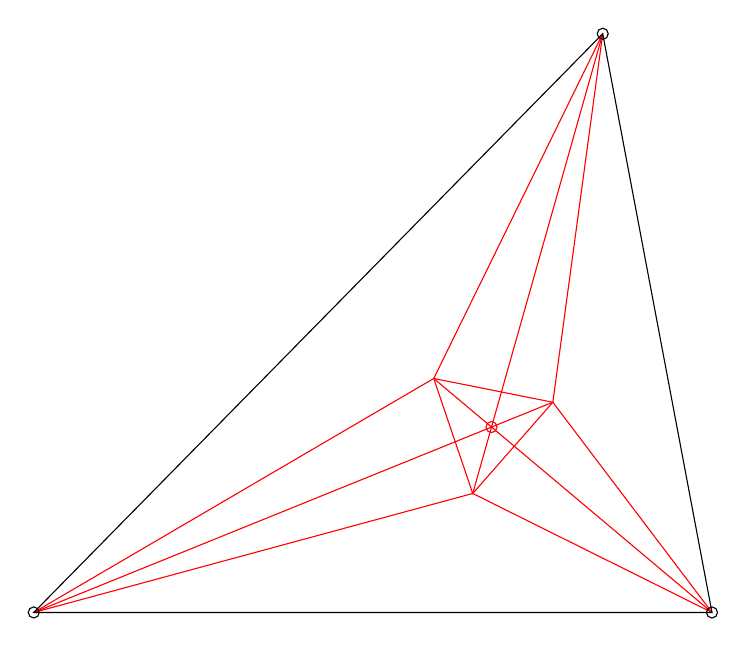
\begin{tikzpicture}[x=1pt,y=1pt]
\draw[red] (172.63,-188.46) -- (201.58,-155.49) -- (158.54,-146.90) -- cycle;
\draw[red] (14.01,-231.45) -- (172.62,-188.46);
\draw[red] (259.08,-231.45) -- (172.63,-188.46);
\draw[red] (259.08,-231.45) -- (201.57,-155.49);
\draw[red] (219.60,-22.34) -- (201.58,-155.49);
\draw[red] (219.60,-22.34) -- (158.54,-146.91);
\draw[red] (158.54,-146.90) -- (14.01,-231.45);
\draw[red] (219.60,-22.34) -- (172.63,-188.46);
\draw[red] (14.01,-231.45) -- (201.57,-155.49);
\draw[red] (259.08,-231.45) -- (158.54,-146.90);
\draw (219.60,-22.34) -- (14.01,-231.45) -- (259.08,-231.45) -- cycle;
\draw (259.08,-231.45) circle (2.00);
\draw (14.01,-231.45) circle (2.00);
\draw (219.60,-22.34) circle (2.00);
\draw[red] (179.42,-164.46) circle (2.00);
\end{tikzpicture}
\end{document}
